\section{Atome}
\subsection{Wasserstoffatom}
\begin{tabular}{p{4cm} p{15cm}}
Schr�dingergleichung	& $\hat{H} = \underbrace{-\frac{\hbar^2}{2m_K} \nabla^2_K}_{E_{kin}\text{ des Kerns}} \underbrace{ -\frac{\hbar^2}{2m_e} \nabla^2_e}_{E_{kin}\text{ des Elektrons}} - \frac{Ze^2}{4\pi\epsilon_0 r} +$ andere Terme\\
Umformung der SG (vgl. Kap. 4.5)	& $\hat{H} = \underbrace{-\frac{\hbar^2}{2M}\nabla^2_{SP}}_{\text{Schwerpunktbew.}} \underbrace{-\frac{\hbar^2}{2\mu}\nabla^2_r-\frac{Ze^s}{4\pi\epsilon_0 r}}_{\text{interne Bewegung}}$\\
vereinfachte SG		& \begin{tabular}[t]{l}
               		  $\hat{H}\Psi = \left( -\frac{\hbar^2}{2\mu} \nabla^2_r - \frac{Ze^2}{4\pi\epsilon_0 r} \right) \Psi = E\Psi$ (QM Coulomb-Potential)\\
			  $\mu = \frac{m_e \cdot m_K}{m_e + m_K} \approx m_e$\\
			  $M = m_e + m_K$\\
			  $Z =$ Kernladungszahl
               		  \end{tabular}\\
Ansatz f�r Eigenfkt.	& $\Psi(r,\theta,\phi) = R(r) \cdot Y_{lm}(\theta,\phi)$\\
L�sungen		& \begin{tabular}[t]{lcll}
			  $R_{n,l}(r)$	& = & $N_{n,l} \exp \left\lbrace -\frac{Zr}{na} \right\rbrace \left( \frac{2Zr}{na} \right)^l L^{2l+1}_{n-l-1}\left( \frac{2Zr}{na} \right)$	&$n = 1,2,...$\\
			  \multicolumn{4}{l}{$a = \frac{m_e}{\mu}a_0;\quad a_0 = \frac{4\pi \epsilon_0 \hbar^2}{m_e e^2} = 0.0529 nm$}\\
        		  $Y_{lm}$	& = & Eigenfkt. des Drehimpulsoperators		& $l = 1,...,(n-1)$\\
					&	&					& $m = -l,-l+1,...l$\\
			  \multicolumn{4}{l}{Superpositionen sind nat�rlich auch wieder L�sungen!}
        		  \end{tabular}\\
Energieeigenwerte	& \begin{tabular}[t]{l}
                 	  $E_{n,l,m} = E_n = -\frac{hcRZ^2}{n^2} = -13.606eV \frac{Z^2}{n^2}$\\
			  $c =$ Lichtgeschwindigkeit; $R = \frac{\mu e^4}{8\epsilon_0^2h^3c}$
                 	  \end{tabular}\\
Entartung		& $g = \sum_{l=0}^{n-1} (2l+1) = n^2$ (Pro $l$ gibt es $2l+1$ $m$)\\
radiale WSKDichte	& \begin{tabular}[t]{ll}
                 	  WSKDichte		&$p_{n,l}(r) dr = |R_{n,l}(r)^2| r^2 dr$\\
			  Radius des Maximums	& $\arg\max_r p_{n,l}(r) = r_{pmax} = \frac{n^2}{Z}a$ (Bohr'scher Atomradius)\\
			  Mittlerer Radius	& $\frac{a}{2Z} \left(3n^2-l(l+1) \right)$
                 	  \end{tabular}\\
Auswahlregeln (Atom�berg�nge) 	& \begin{tabular}[t]{l}
             		  Emission und Absorption von Photonen:\\
			  $\Delta l = l_f - l_i = \pm 1$\\
			  $\Delta j = j_f - j_i = 0, \pm 1\quad j_i = 0 \Rightarrow j_f \neq 0$\\
			  Nur diese �berg�nge k�nnen im Spektrum erscheinen.
             		  \end{tabular}\\
\end{tabular}
\subsection{Mehrelektronenatome}
\begin{tabular}{p{4cm} p{15cm}}
Ein Protonen, zwei Elektron System	& $E_{pot} = -\frac{Ze^2}{4\pi\epsilon_0 r_1} -\frac{Ze^2}{4\pi\epsilon_0 r_2} + \underbrace{\frac{e^2}{4\pi\epsilon_0 r_{12}}}_{Elektron-Elektron-Abstossung}$\\
Permutationsoperator	& \begin{tabular}[t]{l}
                    	  $\hat{P}_{12} \Psi_A(1)\Psi_B(2) = \Psi_A(2)\Psi_B(1)$\\
			  $\left[ \hat{P}, \hat{H} \right] = 0$
                    	  \end{tabular}\\
Satz			& Sei $f(\vec{q}_1, ... , \vec{q}_i, \vec{q}_j,..., \vec{q}_n)$ eine beliebige Funktion. Dann sind die Funktionen $\Psi^{\pm}(\vec{q}_1,...,\vec{q}_n) = f(\vec{q}_1, ... , \vec{q}_i, \vec{q}_j,..., \vec{q}_n) \pm f(\vec{q}_1, ... , \vec{q}_j, \vec{q}_i,..., \vec{q}_n)$ Eigenfunktionen von $\hat{P}_{ij}$ zu den Eigenwerten $\pm 1$\\
Verallgemeinertes Pauli-Prinzip	& \begin{itemize}
                               	  	\item Eigenfkt von $\hat{H}$ sind entweder symmetrisch oder antisymmetrisch bzgl. der Permutation zweier identischer Teilchen (iT).
					\item Eigenfkt m�ssen symmetrisch sein bzgl. einer Permutation zweier iT mit ganzzahligem Spin. (Bosonen)
					\item Eigenfkt m�ssen antisymmetrisch sein bzgl. einer Permutation zweier iT mit halbganzzahligem Spin. (Fermionen, z.B.Elektronen)
                               	  \end{itemize}\\
\multicolumn{2}{p{19cm}}{$\Rightarrow$ Weil Elektronen Fermionen sind, m�ssen die Gesamtwellenfkt. von Mehrelektronenatomen antisymmetrisch sein!}\\
Bahnwellenfunktion Atom			& $\Psi_{Atom}(2,1) =  \Psi_a(2)\Psi_b(1) \pm \Psi_a(1) \Psi_b(2) = \pm \Psi_{Atom}(1,2)\quad$ a,b: Zust�nde; 1,2: Elektronen\\
symmetrische Bahnwellenfunktion		& \begin{tabular}[t]{l}
                               		  	$\Psi_S(1,2) = \Psi_S(2,1)\quad \lim_{a\to b} \Psi_S > 0$\\
						$\Rightarrow$ Elektronen k�nnen einander nahe kommen $\Rightarrow$ Hohe mittlere Abstossungsenergie
                               		  \end{tabular}\\
antisymmetrische Bahnwellenfkt.		& \begin{tabular}[t]{l}
                               		  $\Psi_A(1,2) = -\Psi_A(2,1)\quad \lim_{a\to b} \Psi_A = 0$\\
					  $\Rightarrow$ Elektronen sind einander nie nahe $\Rightarrow$ Niedrige mittlere Abstossungsenergie
                               		  \end{tabular}\\
gleiche Zust�nde		& Die Zust�nde $a,b,c,...$ entsprechen Quantenzust�nden $n,l,m_l$. Sind zwei Elektronen im gleichen Zustand, so ist die antisymmetrische Bahnwellenfkt. $\Psi_A(1,2) = \Psi_a(2)\Psi_a(1) - \Psi_a(1)\Psi_a(2) = 0$ und somit nicht erlaubt.\\
Spins				& Die Spins der beiden Elektronen betragen jeweils $\frac{1}{2}$. Je nach Orientation (parallel, antiparallel) k�nnen sie sich zu 0 oder 1 addieren\\
Spinwellenfkt			& $|\alpha \rangle$ bezeichne die Spinwellenfkt bzgl. $m_s = \tfrac{1}{2}$, $|\beta \rangle$ diejenige bzgl. $m_s = -\tfrac{1}{2}$\\
Gesamtspin $S=0$ (Singulett)	& $\chi_A = \alpha(1)\beta(2)-\alpha(2)\beta(1)\quad M_S = 0$ antisymmetrische Spin-Wellenfkt\\
Gesamtspin $S=1$ (Triplett)	& \begin{tabular}[t]{ll}
                           	   $\chi_S = \alpha(1)\alpha(2)$	& $M_S = 1$\\
				   $\chi_S = \alpha(1)\beta(2) + \alpha(2)\beta(1)$	& $M_S = 0$\\
				   $\chi_S = \beta(1)\beta(2)$	& $M_S = -1$
                           	  \end{tabular} symmetrische Spin-Wellenfkt.\\
				& 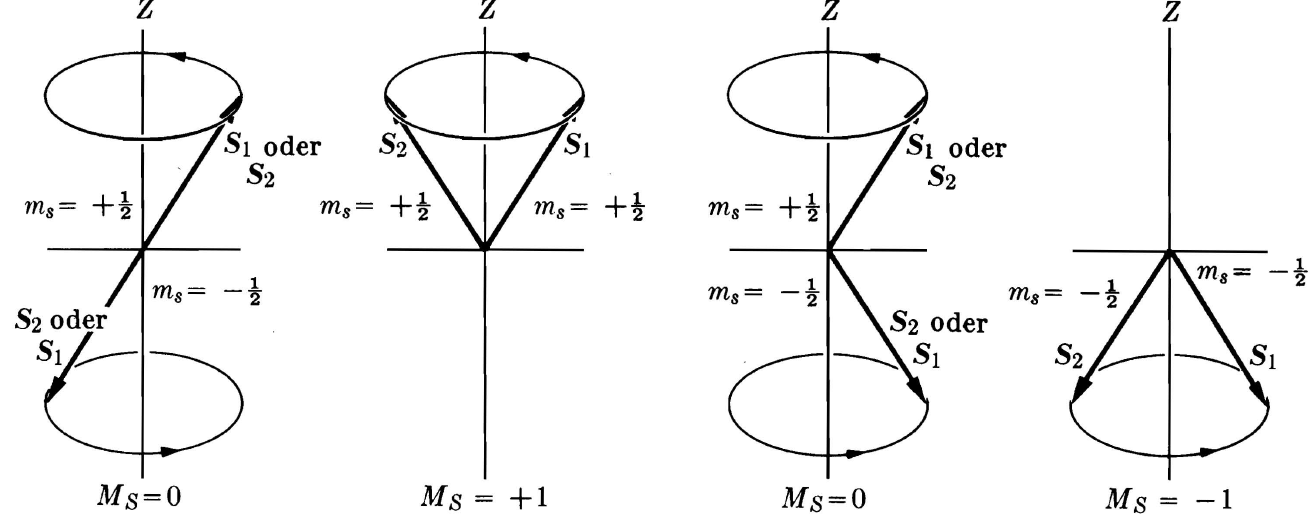
\includegraphics[width = 14cm]{qm_spin.png}\\
\end{tabular}\\\newpage
\begin{tabular}{p{4cm}p{15cm}}
Gesamtwellenfunktion		& \begin{tabular}[t]{p{14cm}}
                    		  $\Psi_{Gesamt} = $ Bahnwellenfkt $\cdot$ Spinwellenfkt = f�r Fermionen immer ANTIsymmetrisch, f�r Bosonen immer symmetrisch. Weil Elektronen Fermionen sind, m�ssen Gesamtwellenfkt. von Atomen immer antisymmetrisch sein.\\
				  Singuletts: symmetrische Bahnwfkt $\cdot$ antisymmetrische Spinwfkt.\\
				  Tripletts: antisymmetrische Bahnwfkt $\cdot$ symmetrische Spinwfkt.\\
				  $\Rightarrow$ Tripletts haben eine tiefere Energie als der Singulett-Zustand (wegen Bahnwfkt, siehe oben)
                    		  \end{tabular}\\

antisymmetrische Gesamtwfkt (Slater-Determinante)	&
				  $\Psi_{abc...} = \frac{1}{\sqrt{N!}} \begin{vmatrix} \varphi_a(1)	& \varphi_b(1)	& \varphi_c(1)	& \dotsc\\
										       \varphi_a(2)	& \varphi_b(2)	& \varphi_c(2)	& \dotsc\\
										       \varphi_a(3)	& \dotsc	& \dotsc	& \dotsc\\
										       \dotsc		& \dotsc	& \dotsc	& \dotsc\\
                   		                                       \end{vmatrix}$\\
Bsp. f�r $1s^2$-Zustand		& \begin{tabular}[t]{l}
				  $\Psi_{\alpha\beta}(1,2) = \frac{1}{\sqrt{2}} \begin{vmatrix} |1s(\vec{r}_1)\alpha(1)\rangle	& |1s(\vec{r}_2)\beta(1)\rangle\\
											        |1s(\vec{r}_1)\alpha(2)\rangle	& |1s(\vec{r}_2)\beta(2)\rangle
                       		                                                \end{vmatrix}$\\
				  $= \frac{1}{\sqrt{2}} (|1s(\vec{r}_1)\alpha(1)\rangle |1s(\vec{r}_2)\beta(2)\rangle - |1s(\vec{r}_1)\alpha(2)\rangle |1s(\vec{r}_2)\beta(1)\rangle)$\\
				  $= \frac{1}{\sqrt{2}} \underbrace{|1s(\vec{r}_1\rangle |1s(\vec{r}_2)\rangle}_{Raumteil} \underbrace{(\alpha(1)\beta(2) - \alpha(2)\beta(1))}_{Spinteil}$
				  \end{tabular}\\
Ausschliessungsprinzip		& Jeder Quantenzustand $(n,l,m_l,m_s)$ kann h�chstens von einem Elektron (allg. Fermionen) eingenommen werden. Die Anzahl Zust�nde ist somit beschr�nkt durch die Abh�ngigkeiten der Quantenzahlen.\\
Besetzungszahl (max. \# $e^-$ f�r ein Atom)	& 2(2l+1)
\end{tabular}
\subsection{Konfigurationen, Terme}
F�r $n$ Elektronen-Atome mit vernachl�ssigbar kleiner Spin-Bahn-Kopplung (gegen�ber Coulomb-WW), so ist das LS-Drehimpulskopplungsschema geeignet.\\
\begin{tabular}{p{4cm}p{5cm}p{5cm}p{5cm}}
Gesamtbahndrehimpuls		& $\hat{\vec{L}} = \sum_{i=1}^n \hat{\vec{l}}_i$	& $\hat{L}_z = \sum_{i=1}^n \hat{l}_{zi}$	& $M_L = \sum_{i=1}^n m_{li}$\\
Gesamtspin			& $\hat{\vec{S}} = \sum_[i=1]^n \hat{\vec{s}}_i$	& $\hat{S}_z = \sum_{i=1}^n \hat{s}_{zi}$	& $M_S = \sum_{i=1}^n m_{si}$\\
Gesamtdrehimpuls		& $\hat{\vec{J}} = \hat{\vec{L}} + \hat{\vec{S}}$	& $\hat{J}_z = \hat{L}_z + \hat{S}_z$\\
				& $J = L+S, L+S-1,..,|L-S|$				& $M_J = M_L + M_S$\\
\end{tabular}
\begin{tabular}{p{4cm}p{15cm}}
Basis f�r leichte Atome		& $|L,M_L\rangle|S,M_S\rangle$ oder $|L,S,J,M_J\rangle$\\
Term				& Menge der $(2S+1)(2L+1)$ Zust�nde zu gegebenen $L,S$\\
Termsymbol			& $^{2S+1}L_J$\\
Regel von Hund			& Im Grundzustand von Atomen hat der resultierende Spin den gr�sstm�glichen Wert, der mit dem Ausschliessungsprinzip vereinbar ist\\
Hundsche Regeln			& Die tiefste Energie hat
				  \begin{enumerate}
               			  	\item der Term mit maximalem S-Wert
					\item der Term mit maximalem L-Wert
					\item kleinsten J-Wert $(J = |L-S|)$ f�r weniger als halbgef�llte Schalen
					\item gr�ssten J-Wert $(J = L+S)$ f�r mehr als halbgef�llte Schalen
               			  \end{enumerate}\\
Elektronenkonfiguration		& $\text{(Hauptquantenzahl)(Bahndrehimpuls)}^{\text{Anz.Elektronen}}\quad $ Bsp: $1s^2 2s^2 2p\quad$ 5$e^- \Rightarrow$ Bor\\
Auswahlregeln (AR)		& \begin{tabular}[t]{rcl}
				    \multicolumn{3}{p{15cm}}{Auswahlregeln f�r elektrische Dipol�berg�nge zwischen zwei Zust�nden $|J'',M_J'',P''\rangle$ und $|J',M_J',P'\rangle$}\\
				     $|J'-J''|$		&$\leq$	& $1 \leq J'+J''$\\
				     $|M_J'-M_J''|$	&$\leq$	& $1$\\
				     $P'P''$		& = 	& $-1$
				  \end{tabular}\\
Zus�tzl. AR f�r LS-Kopplung	& \begin{tabular}[t]{rcl}
				    $|L'-L''|$	& $\leq$	& $1 \leq L'+L''$\\
				    $S'-S''$	& =		& 0\\
				    $l'-l''$	& = 		& $\pm 1$\quad f�r Einelektronen�berg�nge
				  \end{tabular}
\end{tabular}
